\section{The Definite Integral} \label{S:4.3.DefiniteIntegral}

\begin{goals}
\item How does increasing the number of subintervals affect the accuracy of the approximation generated by a Riemann sum?
\item What is the definition of the definite integral of a function $f$ over the interval $[a,b]$?
\item What does the definite integral measure exactly, and what are some of the key properties of the definite integral?
\end{goals}

%--------------------------------------
% SUBSECTION INTRODUCTION
%--------------------------------------
\subsection*{Introduction}

In this chapter, we have computed or approximated the net signed area that is bounded by a function on a given interval. We now give mathematical notation to signify the net signed area.  

\definition{Net Signed Area as The Definite Integral}% DEFINITION
{Let $y=f(x)$ be defined on a closed interval $[a,b]$. The net signed area from $x=a$ to $x=b$ under $f$ is signified by the {\em definite integral} of $f$ on $[a,b]$, which is denoted 
\[ \int_a^b f(x)\ dx.\]
} % end definition

The area definition of the definite integral allows us to compute the definite integral of some simple functions using geometry as we did in section 4.1.

\begin{marginfigure} % MARGIN FIGURE
\margingraphics{figs/4/4-3_TrapArea.pdf}
\caption{The area bounded by $f(x)=2x+1$ and the $x$-axis on the interval $[1,4]$.} \label{fig:4-3_TrapArea}
\end{marginfigure}
  
For instance, if we wish to evaluate the definite integral \\$\ds\int_1^4 (2x+1) \, dx$, we can observe that the region bounded by this function and the $x$-axis is the trapezoid shown in Figure~\ref{fig:4-3_TrapArea}, and by the known formula for the area of a trapezoid, its area is $A = \frac{1}{2}(3+9) \cdot 3 = 18$, so
\[ \int_1^4 (2x+1) \, dx = 18. \]

\pagebreak

\begin{marginfigure} % MARGIN FIGURE
\margingraphics{figs/4/apex_5-2_Def1a.pdf}
\caption{A graph of $f(x) = 2x-4$.} \label{fig:apex_5-2_Def1a}
\end{marginfigure}

\begin{marginfigure}[1cm] % MARGIN FIGURE
\margingraphics{figs/4/apex_5-2_Def1b.pdf}
\caption{A graph of $f(x) = \sqrt{9-x^2}$.} \label{fig:apex_5-2_Def1b}
\end{marginfigure}

\begin{example} % EXAMPLE
Evaluate the following definite integrals using geometry.
\begin{multicols}{2}
\begin{enumerate}[1),leftmargin=*]
\item $\ds \int_{-2}^5 (2x-4) \ dx$
\item $\ds \int_{-3}^3 \sqrt{9-x^2} \ dx$
\end{enumerate}
\end{multicols}

\solution
\begin{enumerate}[1),leftmargin=*]
\item It is useful to sketch the function in the integrand, as shown in Figure \ref{fig:apex_5-2_Def1a}. We see we need to compute the areas of two regions, which we have labeled $R_1$ and $R_2$. Both are triangles, so the area computation is straightforward:
\[ R_1 = \frac{1}{2}(4)(8) = 16 \qquad R_2 = \frac{1}{2}(3)6 = 9.\]
Region $R_1$ lies under the $x$-axis, hence it is counted as negative area (we can think of the height as being ``$-8$''), so 
\[ \int_{-2}^5(2x-4)\ dx = 9-16 = -7. \]

\item Recognize that the integrand of this definite integral is a half circle, as sketched in Figure \ref{fig:apex_5-2_Def1b}, with radius $3$. Thus the area is:
\[ \int_{-3}^3 \sqrt{9-x^2}\ dx = \frac{1}{2}\pi r^2 = \frac{9}{2}\pi. \]
\end{enumerate}
\end{example}   % EXAMPLE

In section 4.2, we found evidence that if we increase the number of rectangles in a Riemann sum, our accuracy of the approximation of the net signed area. We thus explore the natural idea of allowing the number of rectangles to increase without bound in an effort to compute the exact net signed area bounded by a function on an interval.  In addition, it is important to think about the differences among left, right, and middle Riemann sums and the different results they generate as the value of $n$ increases.  As we have done throughout our investigations with area, we begin with functions that are exclusively positive on the interval under consideration.

\pagebreak

\begin{marginfigure}[1cm] % MARGIN FIGURE
\margingraphics{figs/4/4-3_EckApplet.pdf}
\caption{A left Riemann sum with 5 subintervals for the function $f(x) = \frac{3}{1+x^2}$ on the interval $[-5,5]$.  The value of the sum is $L_5 = 7.43076923$.} \label{fig:4-3_EckApplet}
\end{marginfigure}

\begin{marginfigure}[1cm] % MARGIN FIGURE
\margingraphics{figs/4/4-3_EckApplet2.pdf}
\caption{A left Riemann sum with 5 subintervals for the function $f(x) = 2x+1$ on the interval $[1,4]$.  The value of the sum is $L_5 = 16.2$.} \label{fig:4-3_EckApplet2}
\end{marginfigure}

\begin{pa} \label{PA:4.3}
Consider the applet found at \href{http://gvsu.edu/s/aw}{\texttt{http://gvsu.edu/s/aw}}.  There, you will initially see the situation shown in Figure~\ref{fig:4-3_EckApplet}.

Observe that we can change the window in which the function is viewed, as well as the function itself.  Set the minimum and maximum values of $x$ and $y$ so that we view the function on the window where $1 \le x \le 4$ and $-1 \le y \le 12$, where the function is $f(x) = 2x + 1$ (note that you need to enter ``\texttt{2*x+1}'' as the function's formula).  You should see the updated figure shown in Figure~\ref{fig:4-3_EckApplet2}.

Note that the value of the Riemann sum of our choice is displayed in the upper left corner of the window.  Further, by updating the value in the ``Intervals'' window and/or the ``Method'', we can see the different value of the Riemann sum that arises by clicking the ``Compute!'' button.
\ba
	\item Update the applet so that the function being considered is $f(x) = 2x+1$ on $[1,4]$, as directed above.  For this function on this interval, compute $L_{n}$, $M_{n}$,  $R_{n}$ for $n = 10$, $n = 100$, and $n = 1000$.  What do you conjecture is the exact area bounded by $f(x) = 2x+1$ and the $x$-axis on $[1,4]$?
	\item Use basic geometry to determine the exact area bounded by $f(x) = 2x+1$ and the $x$-axis on $[1,4]$.
	\item Based on your work in (a) and (b), what do you observe occurs when we increase the number of subintervals used in the Riemann sum?
	\item Update the applet to consider the function $f(x) = x^2 + 1$ on the interval $[1,4]$ (note that you will want to increase the maximum value of $y$ to at least $17$, and you need to enter ``\texttt{x\^{}2 + 1}'' for the function formula).  Use the applet to compute $L_{n}$, $M_{n}$,  $R_{n}$ for $n = 10$, $n = 100$, and $n = 1000$.  What do you conjecture is the exact area bounded by $f(x) = x^2+1$ and the $x$-axis on $[1,4]$?
	\item Why can we not compute the exact value of the area bounded by $f(x) = x^2+1$ and the $x$-axis on $[1,4]$ using a formula like we did in (b)?
\ea
\end{pa} 
\afterpa % PREVIEW ACTIVITY

%--------------------------------------------------------------------------------------
% SUBSECTION THE FORMAL DEFINITION OF THE DEFINITE INTEGRAL
%--------------------------------------------------------------------------------------
\subsection*{The formal definition of the definite integral} \index{definite integral!definition}

In both examples in Preview Activity~\ref{PA:4.3}, we saw that as the number of rectangles got larger and larger, the values of $L_n$, $M_n$, and $R_n$ all grew closer and closer to the same value.  It turns out that this occurs for any continuous function on an interval $[a,b]$, and even more generally for a Riemann sum using any point $x_{i+1}^*$ in the interval $[x_i, x_{i+1}]$.  Said differently, as we let $n \to \infty$, it doesn't really matter where we choose to evaluate the function within a given subinterval, because
\[ \lim_{n \to \infty} L_n = \lim_{n \to \infty} R_n = \lim_{n \to \infty} M_n = \lim_{n \to \infty} \sum_{i=1}^{n} f(x_i^*) \triangle x.\]
That these limits always exist (and share the same value) for a continuous\footnote{It turns out that a function need not be continuous in order to have a definite integral.  For our purposes, we assume that the functions we consider are continuous on the interval(s) of interest.  It is straightforward to see that any function that is piecewise continuous on an interval of interest will also have a well-defined definite integral.} function $f$ allows us to make the following definition.

\definition{The Definite Integral}{ \label{def:4.3.DefInt} % DEFINITION
The \emph{definite integral} of a continuous function $f$ on the interval $[a,b]$, denoted $\ds \int_a^b f(x) \, dx$, is the real number given by
\[ \int_a^b f(x) \, dx = \lim_{n \to \infty} \sum_{i=1}^{n} f(x_i^*) \triangle x,\]
where $\Delta x = \frac{b-a}{n}$, $x_i = a + i\triangle x$ (for $i = 0, \ldots, n$), and $x_i^*$ satisfies $x_{i-1} \le x_i^* \le x_i$ (for $i = 1, \ldots, n$).
} % end definition

We call the symbol $\int$ the \emph{integral sign}\index{integral sign}, the values $a$ and $b$ the \emph{limits or bounds of integration}\index{limits of integration}\index{bounds of integration}, and the function $f$ the \emph{integrand}\index{integrand}.  The process of determining the real number $\int_a^b f(x) \, dx$ is called \emph{evaluating the definite integral}.  While we will come to understand that there are several different interpretations of the value of the definite integral, for now the most important is that $\int_a^b f(x) \, dx$ measures the net signed area bounded by $y = f(x)$ and the $x$-axis on the interval $[a,b]$.  

\begin{marginfigure} % MARGIN FIGURE
\margingraphics{figs/4/4-2_NegFc.pdf}
\caption{A continuous function $f$ on the interval $[a,d]$.} \label{fig:4-3_NegFc}
\end{marginfigure}

For example, in the notation of the definite integral, if $f$ is the function pictured in Figure~\ref{fig:4-3_NegFc} and $A_1$, $A_2$, and $A_3$ are the exact areas bounded by $f$ and the $x$-axis on the respective intervals $[a,b]$, $[b,c]$, and $[c,d]$, then
\[ \int_a^b f(x) \, dx = A_1, \ \int_b^c f(x) \, dx = -A_2, \ \int_c^d f(x) \, dx = A_3, \]
and
\[ \int_a^d f(x) \, dx = A_1 - A_2 + A_3. \]
We can also use definite integrals to express the change in position and distance traveled by a moving object.  In the setting of a velocity function $v$ on an interval $[a,b]$, it follows from our work above and in preceding sections that the change in position, $s(b) - s(a)$, is given by
\[ s(b) - s(a) = \int_a^b v(t) \, dt. \]
If the velocity function is nonnegative on $[a,b]$, then $\int_a^b v(t) \,dt$ tells us the distance the object traveled.  When velocity is sometimes negative on $[a,b],$ the areas bounded by the function on intervals where $v$ does not change sign can be found using integrals, and the sum of these values will tell us the distance the object traveled. 

If we wish to compute the value of a definite integral using the definition, we have to take the limit of a sum.  While this is possible to do in select circumstances, it is also tedious and time-consuming; therefore, we typically take the limit of only relatively simple sums.  

\begin{example} % EXAMPLE
Use limits to compute the exact value of
\[ A = \int_0^4 (4x-x^2) \ dx, \]
supposing that 
\[ A \approx \frac{32}{3}\left(1-\frac{1}{n^2}\right). \]

\solution Taking the limit as $n \to \infty$, 
\[ A = \lim_{n \to \infty} \frac{32}{3} \left( 1-\frac{1}{n^2} \right) = \frac{32}{3}. \]
\end{example} % EXAMPLE

\begin{example} % EXAMPLE
Find a formula that approximates $\ds \int_{-2}^3 (5x+2) \ dx$ using $R_n$; then take the limit as $n \to \infty$ to find the exact area.

\solution We have $\ds \Delta x = \frac{3 - (-2)}{n} = \frac{5}{n}$ and $\ds x_i = -2 + \frac{5}{n}i$,
and we construct the Riemann sum and compute its value using summation formulas.
\begin{align*}
\int_{-2}^3 (5x+2) \ dx & \approx \sum_{i=1}^{n} f(x_i) \Delta x \\
&=	\sum_{i=1}^{n} f(-2 + i \Delta x )\Delta x \\
&=	\sum_{i=1}^{n} \big( 5 (-2 + i \Delta x ) + 2 \big) \Delta x \\
&=	\Delta x \sum_{i=1}^{n} \left[ \left( 5 \Delta x \right) i - 8 \right] \\
&=	\Delta x \left[ 5 \Delta x \sum_{i=1}^{n} (i) - \sum_{i=1}^{n}8 \right] \\
&= \frac{5}{n} \left[ \frac{25}{n} \cdot \frac{n(n+1)}{2} - 8 \cdot n \right]  \\
&= \frac{125n(n+1)}{2n^2} - 40.
\end{align*}

%\marginfigure{.55}{Approximating $\int_{-2}^3 (5x+2)\ dx$ using the Midpoint Rule and 10 evenly spaced subintervals in Example \ref{ex_rie8}.}{fig:rie8}{figures/figrie8}
% this picture needs corrected

Taking the limit we get 
\[ \int_{-2}^{3} (5x+2) \; dx = \lim_{n \to \infty} \frac{125n(n+1)}{2n^2} - 40 = \frac{45}{2}. \]
\end{example}  % EXAMPLE

%\begin{marginfigure} % MARGIN FIGURE
%\margingraphics{figs/4/apex_5-3_Area3R.pdf}
%\caption{Approximating $\int_{-1}^5 x^3\ dx$ using $R_n$.} \label{fig:apex_5-3_Area3R}
%\end{marginfigure}

\begin{activity} \label{A:4.3.4} % ACTIVITY
Use the properties of summations and limits to find the exact net area of the region underneath the function $x^3$ on the interval $[-1,5]$.

\ba
\item Sketch a graph of $f(x) = x^3$.
\item Find formulas for $\Delta x$ and $x_i$ in terms of $n$.
\item Generate an approximation for $\int_{-1}^{5} x^3 \ dx$ in terms of $n$.
\item Using the approximation you found in (c), take the limit as $n \to \infty$ to find the exact net area.
\ea
\end{activity} % EXAMPLE %%% Make this example an activity!!!

In Section~\ref{S:4.4.FTC}, we will learn the Second Part of the Fundamental Theorem of Calculus, a theorem that provides an analytical process for evaluating a large class of definite integrals.  This will enable us to determine the exact net signed area bounded by a continuous function and the $x$-axis in many circumstances, including examples such as $\ds\int_1^4 (x^2 + 1) \, dx$, which we approximated by Riemann sums in Preview Activity~\ref{PA:4.3}.

For now, our goal is to understand the meaning and properties of the definite integral, rather than how to actually compute its value using ideas in calculus.  Thus, we temporarily rely on the net signed area interpretation of the definite integral and observe that if a given curve produces regions whose areas we can compute exactly through known area formulas, we can thus compute the exact value of the integral.

\begin{marginfigure}[6cm] % MARGIN FIGURE
\margingraphics{figs/4/activity_4-3-1.pdf}
\caption{A function $g$ that is piecewise defined; each piece of the function is part of a circle or part of a line.} \label{fig:activity_4-3-1}
\end{marginfigure}

\begin{activity} \label{A:4.3.1}  Use known geometric formulas and the net signed area interpretation of the definite integral to evaluate each of the definite integrals below.
\ba
	\item $\ds \int_0^1 3x \, dx$
	\item $\ds \int_{-1}^4 (2-2x) \, dx$
	\item $\ds \int_{-1}^1 \sqrt{1-x^2} \, dx$
	\item $\ds \int_{-3}^4 g(x) \, dx$, where $g$ is the function pictured in Figure~\ref{fig:activity_4-3-1}.  Assume that each portion of $g$ is either part of a line or part of a circle.
\ea
%\begin{figure}[h]
%\begin{center}
%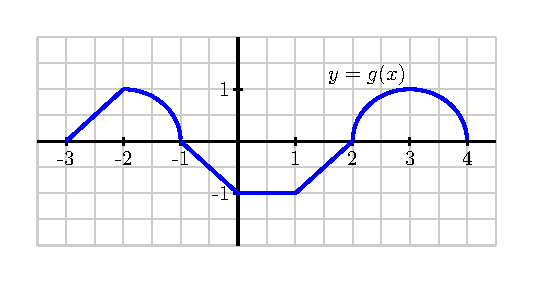
\includegraphics{figures/4_3_Act1.eps}
%\caption{A function $g$ that is piecewise defined; each piece of the function is part of a circle or part of a line.} \label{F:4.3.Act1}
%\end{center}
%\end{figure}
\end{activity}
\begin{smallhint}
\ba
	\item Sketch the region bounded by $y = 3x$ and the $x$-axis on $[0,1]$.
	\item Sketch the region bounded by $y = 2-2x$ and the $x$-axis on $[-1,4]$.
	\item Observe that $y = \sqrt{1-x^2}$ is the top half the circle whose equation is $x^2 + y^2 = 1$.
	\item Use known formulas for the area of a triangle, square, or circle appropriately.
\ea
\end{smallhint}
\begin{bighint}
\ba
	\item Sketch the region bounded by $y = 3x$ and the $x$-axis on $[0,1]$ and observe that it forms a familiar geometric shape.
	\item Sketch the region bounded by $y = 2-2x$ and the $x$-axis on $[-1,4]$; think carefully about the role of signed area in determining the value of the integral, and subdivide the problem by considering regions on which the curve is positive and negative.
	\item Observe that $y = \sqrt{1-x^2}$ is the top half the circle whose equation is $x^2 + y^2 = 1$.
	\item Use known formulas for the area of a triangle, square, or circle appropriately.  Keep in mind the role of signed area when dealing with the portions of the region that lie below the $x$-axis.
\ea
\end{bighint}
\begin{activitySolution}
\ba
	\item Because $y = 3x$ and the $x$-axis bound a triangle with base of length 1 and height $3$ on the interval $[0,1]$, it follows that 
	$$\ds \int_0^1 3x \, dx = \frac{1}{2} \cdot 1 \cdot 3 = \frac{3}{2}.$$
	\item For $\ds \int_{-1}^4 (2-2x) \, dx$, we first sketch the region bounded by the function, as shown below.
	\begin{center}
	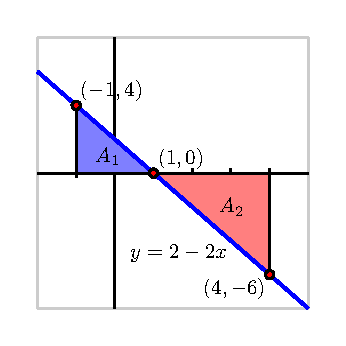
\includegraphics{figures/4_3_Act1bSoln.eps}
	\end{center}
	The line creates two triangles, one with area $A_1 = \frac{1}{2} \cdot 2 \cdot 4 = 4$ and the other with area $A_2 = \frac{1}{2} \cdot 3 \cdot 6 = 9$.  Since the latter area corresponds to a region below the $x$-axis, we associate a negative sign to it, and hence find that
	$$\int_{-1}^4 (2-2x) \, dx = A_1 - A_2 = 4 - 9 = -5.$$
	\item For $\ds \int_{-1}^1 \sqrt{1-x^2} \, dx$, we simply observe that this function is the top half of a circle of radius 1, and thus the bounded region is a semicircle of radius 1, thus having an area of $\frac{\pi}{2}$.  Therefore,
	$$\ds \int_{-1}^1 \sqrt{1-x^2} \, dx = \frac{\pi}{2}.$$
	\item Finally, for $\ds \int_{-3}^4 g(x) \, dx$, where $g$ is the function pictured in Figure~\ref{F:4.3.Act1}, we consider the function on seven consecutive subintervals of length 1.  Observe that on $[-3,-2]$, the bounded area is $\frac{1}{2}$.  On $[-2,-1]$, the area is $\frac{1}{4} \pi$.  Similarly, on the next five subintervals of length 1, the areas bounded are respectively $\frac{1}{2}$, $1$, $\frac{1}{2}$, $\frac{1}{4} \pi$, and $\frac{1}{4} \pi$.  Thus, the value of the integral is
	$$\int_{-3}^4 g(x) \, dx = \frac{1}{2} + \frac{\pi}{4} - \frac{1}{2} - 1 - \frac{1}{2} + \frac{\pi}{4} + \frac{\pi}{4} = \frac{3\pi}{4} - \frac{3}{2},$$
	which is approximately 0.8562.
\ea
\end{activitySolution}
\aftera % ACTIVITY

%-----------------------------------------------------------------------------
% SUBSECTION SOME PROPERTIES OF THE DEFINITE INTEGRAL
%-----------------------------------------------------------------------------
\subsection*{Some properties of the definite integral}

With the perspective that the definite integral of a function $f$ over an interval $[a,b]$ measures the net signed area bounded by $f$ and the $x$-axis over the interval, we naturally arrive at several different standard properties of the definite integral.  In addition, it is helpful to remember that the definite integral is defined in terms of Riemann sums that fundamentally consist of the areas of rectangles.

\concept{Properties of the Definite Integral} % CONCEPT
{Let $f$ and $g$ be defined on a closed interval $I$ that contains the values $a$, $b$ and $c$, and let $k$ be a constant. The following hold:\index{integration!definite!properties}\index{definite integral!properties}
\begin{enumerate}[1)]
\item $\ds \int_a^a f(x) \ dx = 0$

\item $\ds \int_a^b f(x) \ dx + \int_b^c f(x)\ dx = \int_a^cf(x)\ dx$

\item $\ds \int_b^a f(x) \ dx = -\int_a^b f(x)\ dx$

\item $\ds \int_a^b k \cdot f(x) \ dx = k \cdot \int_a^b f(x) \ dx$

\item $\ds \int_a^b \big( f(x)\pm g(x) \big) \ dx = \int_a^b f(x) \ dx \pm \int_a^b g(x) \ dx$
\end{enumerate}
} % end concept

We give a brief justification the properties here.
\begin{enumerate}[1)]
\item If we consider the definite integral $\int_a^a f(x) \, dx$ for any real number $a$, it is evident that no area is being bounded because the interval begins and ends with the same point.  Hence, this definite integral is $0$.
   
\begin{marginfigure} % MARGIN FIGURE
\margingraphics{figs/4/4-3_AddProp.pdf}
\caption{A continuous function $f$ on the interval $[a,d]$.} \label{fig:4-3_AddProp}
\end{marginfigure}
		
\item This states that total area is the sum of the areas of subregions. In Figure~\ref{fig:4-3_AddProp}, we see that  \small
$$\int_a^b f(x) \, dx = A_1, \ \int_b^c f(x) \, dx = A_2, \ \mbox{and} \ \int_a^c f(x) \, dx = A_1 + A_2.$$ \normalsize
It is important to note that this still holds true even if $a<b<c$ is not true. 

\item This result makes sense because if we integrate from $a$ to $b$, then in the defining Riemann sum $\triangle x = \frac{b-a}{n}$, while if we integrate from $b$ to $a$, $\triangle x = \frac{a-b}{n} = -\frac{b-a}{n}$, and this is the only change in the sum used to define the integral.

\item First, let's consider the situation pictured in Figure~\ref{fig:4-3_ConstMultb}, where we examine the effect of multiplying a function  in Figure~\ref{fig:4-3_ConstMulta} by a factor of $2$ on the area it bounds with the $x$-axis.  Because multiplying the function by $2$ doubles its height at every $x$-value, we see that if we consider a typical rectangle from a Riemann sum, the difference in area comes from the changed height of the rectangle:  $f(x_i)$ for the original function, versus $2f(x_i)$ in the doubled function, in the case of left sum.  Hence, we see that for the pictured rectangles with areas $A$ and $B$, it follows $B = 2A$.  As this will happen in every such rectangle, regardless of the value of $n$ and the type of sum we use, we see that in the limit, the area of the red region bounded by $y = 2f(x)$ will be twice that of the area of the blue region bounded by $y = f(x)$.  As there is nothing special about the value $2$ compared to an arbitrary constant $k$, it turns out that the general principle holds.

\begin{marginfigure}[-9cm] % MARGIN FIGURE
\begin{center}
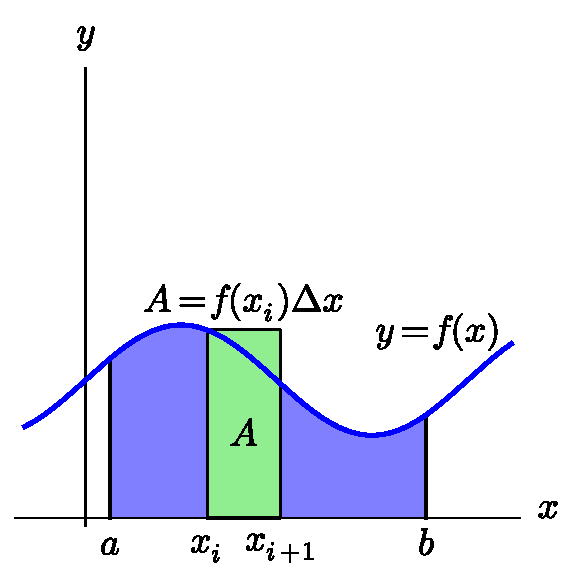
\includegraphics[scale=.5]{figs/4/4-3_ConstMulta.pdf}
\caption{The area bounded by $y = f(x)$ on $[a,b]$.} \label{fig:4-3_ConstMulta}
\end{center}
\end{marginfigure}

\begin{marginfigure}[-1cm] % MARGIN FIGURE
\begin{center}
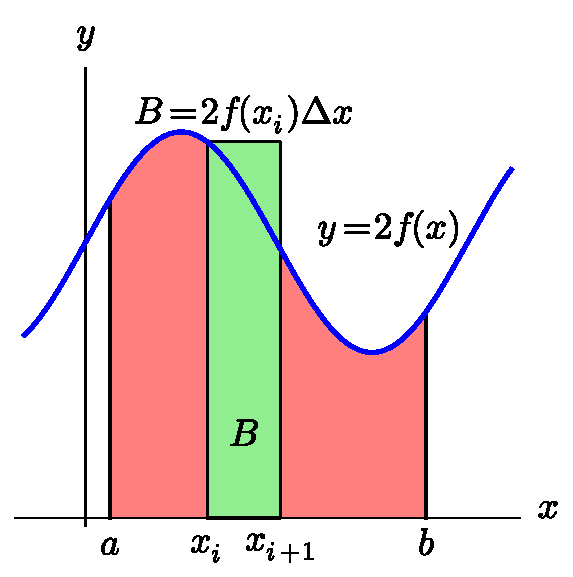
\includegraphics[scale=.5]{figs/4/4-3_ConstMultb.pdf}
\caption{The area bounded by $y = 2f(x)$ on $[a,b]$.} \label{fig:4-3_ConstMultb}
\end{center}
\end{marginfigure}

\item Finally, we see a similar situation geometrically with the sum of two functions $f$ and $g$. In particular, as shown in Figure~\ref{fig:4-3_Sum}, if we take the sum of two functions $f$ and $g$, at every point in the interval, the height of the function $f+g$ is given by $(f+g)(x_i) = f(x_i) + g(x_i)$, which is the sum of the individual function values of $f$ and $g$ (taken at left endpoints).  Hence, for the pictured rectangles with areas $A$, $B$, and $C$, it follows that $C = A + B$, and because this will occur for every such rectangle, in the limit the area of the gray region will be the sum of the areas of the blue and red regions.  

\begin{figure*} % FULLWIDTH FIGURE
\begin{flushright}
\captionsetup[subfigure]{labelformat=empty}
\subfloat{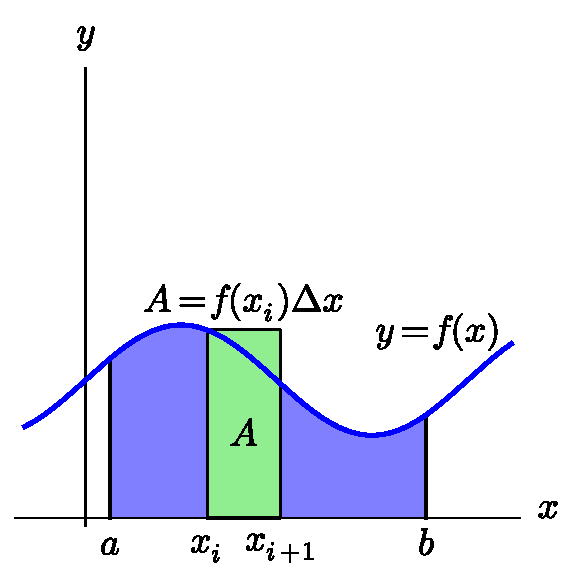
\includegraphics[scale=.5]{figs/4/4-3_Suma.pdf}}
\hspace{.25cm}
\subfloat{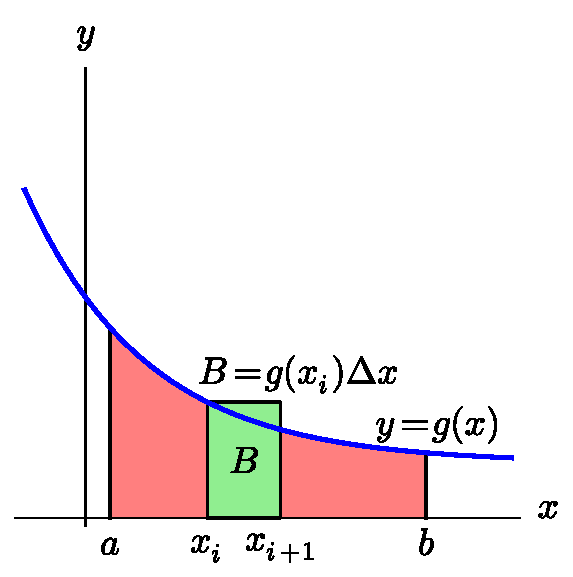
\includegraphics[scale=.5]{figs/4/4-3_Sumb.pdf}}
\hspace{.25cm}
\subfloat{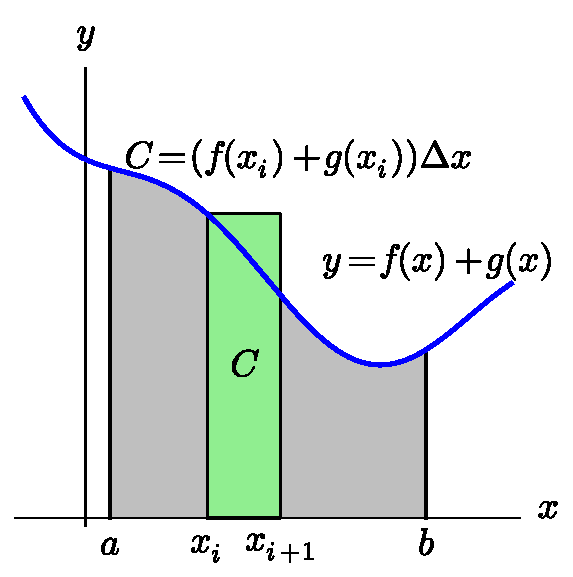
\includegraphics[scale=.5]{figs/4/4-3_Sumc.pdf}}
\caption{The areas bounded by $y = f(x)$ and $y = g(x)$ on $[a,b]$, as well as the area bounded by $y = f(x) + g(x)$.}
\label{fig:4-3_Sum}
\end{flushright}
\end{figure*}
\end{enumerate}

\begin{activity} \label{A:4.3.2}  Suppose that the following information is known about the functions $f$, $g$, $x^2$, and $x^3$:
\begin{itemize}
	\item $\ds \int_0^2 f(x) \, dx = -3$; $\ds \int_2^5 f(x) \, dx = 2$
	\item $\ds \int_0^2 g(x) \, dx = 4$; $\ds \int_2^5 g(x) \, dx = -1$
	\item $\ds \int_0^2 x^2 \, dx = \frac{8}{3}$; $\ds \int_2^5 x^2 \, dx = \frac{117}{3}$
	\item $\ds \int_0^2 x^3 \, dx = 4$; $\ds \int_2^5 x^3 \, dx = \frac{609}{4} $
\end{itemize}
Use the provided information and the rules discussed in the preceding section to evaluate each of the following definite integrals.
\bmtwo\ba
	\item $\ds \int_5^2 f(x) \, dx$
	\item $\ds \int_0^5 g(x) \, dx$
	\item $\ds \int_0^5 (f(x) + g(x))\, dx$
	\item $\ds \int_2^5 (3x^2 - 4x^3) \, dx$
	\item $\ds \int_5^0 (2x^3 - 7g(x)) \, dx$
\ea\emtwo
\end{activity}
\begin{smallhint}
\ba
	\item Note that the value of $\int_2^5 f(x) \, dx$ is given.
	\item Use the values of $\int_0^2 g(x) \,dx$ and $\int_2^5 g(x) \,dx$.
	\item First find $\int_0^5 f(x) \, dx$ and $\int_0^5 g(x) \, dx$.
	\item Use the sum and constant multiple rules.
	\item First write $\int_5^0 (2x^3 - 7g(x)) \, dx = -\int_0^5 (2x^3 - 7g(x)) \, dx$.
\ea
\end{smallhint}
\begin{bighint}
\ba
	\item Note that the value of $\int_2^5 f(x) \, dx$ is given.
	\item Use the values of $\int_0^2 g(x) \,dx$ and $\int_2^5 g(x) \,dx$.
	\item First find $\int_0^5 f(x) \, dx$ and $\int_0^5 g(x) \, dx$; then use the sum rule.
	\item Use the sum and constant multiple rules.  Observe that $\int_2^5 (3x^2 - 4x^3) \, dx = 3\int_2^5 x^2 \, dx - 4\int_2^5 x^3 \, dx.$
	\item First write $\int_5^0 (2x^3 - 7g(x)) \, dx = -\int_0^5 (2x^3 - 7g(x)) \, dx$.  Then use the sum and constant multiple rules.
\ea
\end{bighint}
\begin{activitySolution}
\ba
	\item Note that the value of $\int_2^5 f(x) \, dx$ is given, and thus
	$$\int_5^2 f(x) \,dx = -\int_2^5 f(x) \, dx = -2.$$
	\item Since $\int_0^2 g(x) \,dx = 4$ and $\int_2^5 g(x) \,dx = -1$, we have
	$$\int_0^5 g(x) \,dx = \int_0^2 g(x) \,dx + \int_2^5 g(x) \,dx = 4 + (-1) = 3.$$
	\item First, using work from and similar to that in (c), we find $\int_0^5 f(x) \, dx = -3 + 2 = -1$ and $\int_0^5 g(x) \, dx = 3$, thus by the sum rule,
	$$\int_0^5 (f(x) + g(x))\, dx = \int_0^5 f(x)\, dx + \int_0^5 g(x)\, dx = -1 + 3 = 2.$$
	\item By the sum and constant multiple rules,
	$$\int_2^5 (3x^2 - 4x^3) \, dx = 3\int_2^5 x^2 \, dx - 4\int_2^5 x^3 \, dx = 3 \cdot \frac{8}{3} - 4 \frac{609}{4} = 8 - 609 = -608.$$
	\item First, we write $\int_5^0 (2x^3 - 7g(x)) \, dx = -\int_0^5 (2x^3 - 7g(x)) \, dx$.  Then, using the sum and constant multiple rules, it follows
\begin{eqnarray*}
	\int_5^0 (2x^3 - 7g(x)) \, dx & = & -\int_0^5 (2x^3 - 7g(x)) \, dx \\
					& = & -\left(2 \int_0^5 x^3 \, dx - 7 \int_0^5 g(x) \,dx \right) \\
					& = & -2 \left(\frac{8}{3} + \frac{117}{3}\right)  + 7 \left(4 +  (-1))\right) \\
					& = & -\frac{250}{3} + 21 \\
					& = & -\frac{187}{3}.
\end{eqnarray*}
\ea
\end{activitySolution}
\aftera % ACTIVITY

%-------------
% SUMMARY
%-------------
\begin{summary}
\item Any Riemann sum of a continuous function $f$ on an interval $[a,b]$ provides an estimate of the net signed area bounded by the function and the horizontal axis on the interval.  Increasing the number of subintervals in the Riemann sum improves the accuracy of this estimate, and letting the number of subintervals increase without bound results in the values of the corresponding Riemann sums approaching the exact value of the enclosed net signed area.

\item When we take the just described limit of Riemann sums, we arrive at what we call the definite integral of $f$ over the interval $[a,b]$.  In particular, the symbol $\int_a^b f(x) \, dx$ denotes the definite integral of $f$ over $[a,b]$, and this quantity is defined by the equation
\[ \int_a^b f(x) \, dx = \lim_{n \to \infty} \sum_{i=1}^{n} f(x_i^*) \triangle x, \]
where $\triangle x = \frac{b-a}{n}$, $x_i = a + i\triangle x$ (for $i = 0, \ldots, n$), and $x_i^*$ satisfies $x_{i-1} \le x_i^* \le x_i$ (for $i = 1, \ldots, n$).

\item The definite integral $\int_a^b f(x) \,dx$ measures the exact net signed area bounded by $f$ and the horizontal axis on $[a,b]$. %; in addition, the value of the definite integral is related to what we call the average value of the function on $[a,b]$: $f_{\mbox{\tiny{AVG}}[a,b]} = \frac{1}{b-a} \cdot \int_a^b f(x) \, dx.$  
In the setting where we consider the integral of a velocity function $v$, $\int_a^b v(t) \,dt$ measures the exact change in position of the moving object on $[a,b]$; when $v$ is nonnegative, $\int_a^b v(t) \,dt$ is the object's distance traveled on $[a,b]$.  

\item The definite integral is a sophisticated sum, and thus has some of the same natural properties that finite sums have.  Perhaps most important of these is how the definite integral respects sums and constant multiples of functions, which can be summarized by the rule
\[ \ds \int_a^b [c f(x) \pm k g(x)] \,dx = c \int_a^b f(x) \,dx \pm k \int_a^b g(x) \,dx \]
where $f$ and $g$ are continuous functions on $[a,b]$ and $c$ and $k$ are arbitrary constants.
\end{summary}

\clearpage

%--------------
% EXERCISES
%--------------
\begin{adjustwidth*}{}{-2.25in}
\textbf{{\large Exercises}}
\setlength{\columnsep}{25pt}
\begin{multicols*}{2}
\noindent Terms and Concepts \small
\begin{enumerate}[1)]
\item What is ``total signed area''?
\item What is ``displacement''?
\item What is $\ds \int_3^3 \sin (x)\ dx$?
\item Give a single definite integral that has the same value as 

$\ds \int_0^1(2x+3)\ dx + \int_1^2 (2x+3)\ dx$.
\end{enumerate} 

\noindent {\normalsize Problems} \small

\noindent{\bf In exercises 5--9, a graph of a function $f(x)$ is given.  Using the geometry of the graph, evaluate the definite integral.}

\begin{enumerate}[1),resume]
\item \noindent
\begin{minipage}{\linewidth}
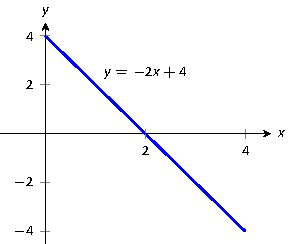
\includegraphics[scale=.8]{figures/fig05_02_ex_05}
\end{minipage}
\bmtwo
\begin{enumerate}
\item		$\ds \int_0^1 (-2x+4)\ dx$
\item		$\ds \int_0^2 (-2x+4)\ dx$
\item		$\ds \int_0^3 (-2x+4)\ dx$
\item		$\ds \int_1^3 (-2x+4)\ dx$
\item		$\ds \int_2^4 (-2x+4)\ dx$
\item		$\ds \int_0^1 (-6x+12)\ dx$
\end{enumerate}
\emtwo

\item\noindent
\begin{minipage}{\linewidth}
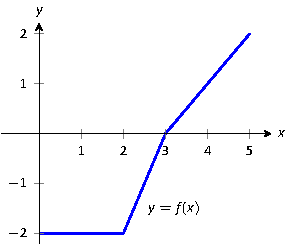
\includegraphics[scale=.8]{figures/fig05_02_ex_06}
\end{minipage}
\bmtwo
\begin{enumerate}
\item		$\ds \int_0^2 f(x)\ dx$
\item		$\ds \int_0^3 f(x)\ dx$
\item		$\ds \int_0^5 f(x)\ dx$
\item		$\ds \int_2^5 f(x)\ dx$
\item		$\ds \int_5^3 f(x)\ dx$
\item		$\ds \int_0^3 -2f(x)\ dx$
\end{enumerate}
\emtwo

\item \noindent
\begin{minipage}{\linewidth}
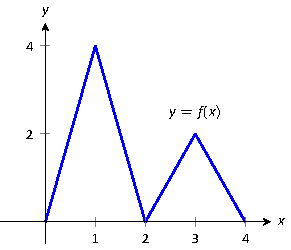
\includegraphics[scale=.8]{figures/fig05_02_ex_07}
\end{minipage}
\bmtwo
\begin{enumerate}
\item		$\ds \int_0^2 f(x)\ dx$
\item		$\ds \int_2^4 f(x)\ dx$
\item		$\ds \int_2^4 2f(x)\ dx$
\item		$\ds \int_0^1 4x\ dx$
\item		$\ds \int_2^3 (2x-4)\ dx$
\item		$\ds \int_2^3 (4x-8)\ dx$
\end{enumerate}
\emtwo

\item \noindent
\begin{minipage}{\linewidth}
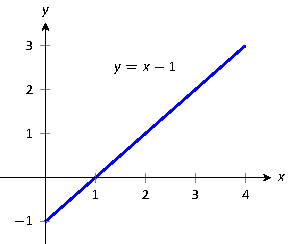
\includegraphics[scale=.8]{figures/fig05_02_ex_08}
\end{minipage}
\bmtwo
\begin{enumerate}
\item		$\ds \int_0^1 (x-1)\ dx$
\item		$\ds \int_0^2 (x-1)\ dx$
\item		$\ds \int_0^3 (x-1)\ dx$
\item		$\ds \int_2^3 (x-1)\ dx$
\item		$\ds \int_1^4 (x-1)\ dx$
\item		$\ds \int_1^4 \big((x-1)+1\big)\ dx$
\end{enumerate}
\emtwo

\item \noindent
\begin{minipage}{\linewidth}
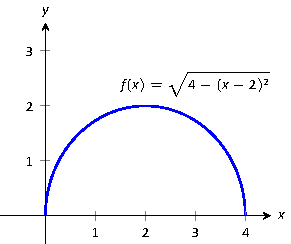
\includegraphics[scale=.8]{figures/fig05_02_ex_09}
\end{minipage}
\bmtwo
\begin{enumerate}
\item		$\ds \int_0^2 f(x)\ dx$
\item		$\ds \int_2^4 f(x)\ dx$
\item		$\ds \int_0^4 f(x)\ dx$
\item		$\ds \int_0^4 5f(x)\ dx$
\end{enumerate}
\emtwo
\end{enumerate}

\noindent{\bf In exercises 10--13, a graph of a function $f(x)$ is given; the numbers inside the shaded regions give the area of that region.  Evaluate the definite integrals using this area information.}

\begin{enumerate}[1),resume]
\item \noindent
\begin{minipage}{\linewidth}
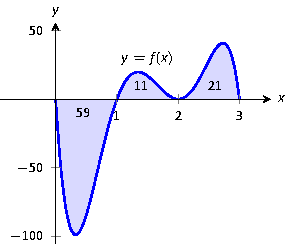
\includegraphics[scale=.8]{figures/fig05_02_ex_10}
\end{minipage}
\bmtwo
\begin{enumerate}
\item		$\ds \int_0^1 f(x)\ dx$
\item		$\ds \int_0^2 f(x)\ dx$
\item		$\ds \int_0^3 f(x)\ dx$
\item		$\ds \int_1^2 -3f(x)\ dx$
\end{enumerate}
\emtwo


\end{enumerate}

%------------------------------------------
% END OF EXERCISES ON FIRST PAGE
%------------------------------------------
\end{multicols*}
\end{adjustwidth*}

\clearpage

\begin{adjustwidth*}{}{-2.25in}
\setlength{\columnsep}{25pt}
\begin{multicols*}{2}\small

\begin{enumerate}[1),start=11]
\item \noindent
\begin{minipage}{\linewidth}
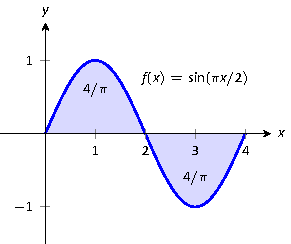
\includegraphics[scale=.8]{figures/fig05_02_ex_11}
\end{minipage}
\bmtwo
\begin{enumerate}
\item		$\ds \int_0^2 f(x)\ dx$
\item		$\ds \int_2^4 f(x)\ dx$
\item		$\ds \int_0^4 f(x)\ dx$
\item		$\ds \int_0^1 f(x)\ dx$
\end{enumerate}
\emtwo

\item \noindent
\begin{minipage}{\linewidth}
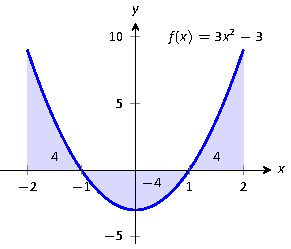
\includegraphics[scale=.8]{figures/fig05_02_ex_12}
\end{minipage}
\bmtwo
\begin{enumerate}
\item		$\ds \int_{-2}^{-1} f(x)\ dx$
\item		$\ds \int_1^2 f(x)\ dx$
\item		$\ds \int_{-1}^1 f(x)\ dx$
\item		$\ds \int_0^1 f(x)\ dx$
\end{enumerate}
\emtwo

\item \noindent
\begin{minipage}{\linewidth}
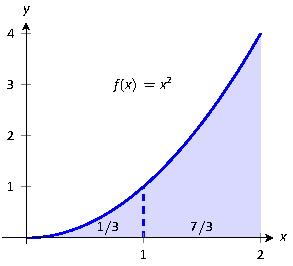
\includegraphics[scale=.8]{figures/fig05_02_ex_13}
\end{minipage}
\bmtwo
\begin{enumerate}
\item		$\ds \int_{0}^{2} 5x^2\ dx$
\item		$\ds \int_0^2 (x^2+3)\ dx$
\item		$\ds \int_{1}^3 (x-1)^2\ dx$
\item		$\ds \int_2^4 \big((x-2)^2+5\big)\ dx$
\end{enumerate}
\emtwo

\end{enumerate}

\noindent{\bf In exercises 14--17, let
\bmtwo
\begin{itemize}
\item $\ds \int_0^2 f(x) \ dx = 5,$
\item $\ds \int_0^3 f(x) \ dx = 7,$
\item $\ds \int_0^2 g(x) \ dx = -3$, and
\item $\ds \int_2^3 g(x) \ dx = 5.$
\end{itemize}
\emtwo
Use these values to evaluate the given definite integrals.}

\begin{enumerate}[1),resume]
\item $\ds \int_0^2 \big(f(x)+g(x)\big) \ dx$
\item $\ds \int_0^3 \big(f(x)-g(x)\big) \ dx$
\item $\ds \int_2^3 \big(3f(x)+2g(x)\big) \ dx$
\item Find values for $a$ and $b$ such that 

$\ds \int_0^3 \big(af(x)+bg(x)\big) \ dx=0$
\end{enumerate}

\noindent{\bf In exercises 18--21, let 
\bmtwo
\begin{itemize}
\item $\ds \int_0^3 s(t) \ dt = 10,$
\item $\ds \int_3^5 s(t) \ dx = 8,$
\item $\ds \int_3^5 r(t) \ dx = -1$, and
\item $\ds \int_0^5 r(t) \ dx = 11.$
\end{itemize}
\emtwo
Use these values to evaluate the given definite integrals.}

\begin{enumerate}[1),resume]
\item $\ds \int_0^3 \big(s(t) + r(t)\big)\ dt$
\item $\ds \int_5^0 \big(s(t) - r(t)\big)\ dt$
\item $\ds \int_3^3 \big(\pi s(t) - 7r(t)\big)\ dt$
\item Find values for $a$ and $b$ such that 

$\ds \int_0^5 \big(ar(t)+bs(t)\big) \ dt=0$

 \item The velocity of an object moving along an axis is given by the piecewise linear function $v$ that is pictured below.  Assume that the object is moving to the right when its velocity is positive, and moving to the left when its velocity is negative.  Assume that the given velocity function is valid for $t = 0$ to $t = 4$.
\begin{center}
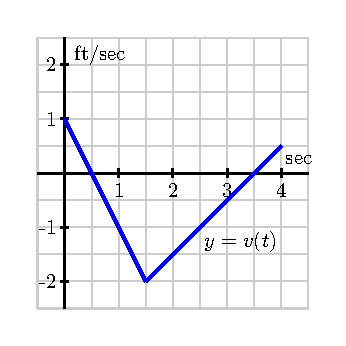
\includegraphics[scale=.75]{figures/4_3_Ez1.eps}
\end{center}
	\ba
		\item Write an expression involving definite integrals whose value is the total change in position of the object on the interval $[0,4]$.
		\item Use the provided graph of $v$ to determine the value of the total change in position on $[0,4]$.
		\item Write an expression involving definite integrals whose value is the total distance traveled by the object on $[0,4]$.  What is the exact value of the total distance traveled on $[0,4]$?
		\item What is the object's exact average velocity on $[0,4]$?
		\item Find an algebraic formula for the object's position function on $[0, 1.5]$ that satisfies $s(0) = 0$.
	\ea
\end{enumerate}

%---------------------------------------------
% END OF EXERCISES ON SECOND PAGE
%---------------------------------------------
\end{multicols*}
\end{adjustwidth*}

\afterexercises 

\cleardoublepage